\documentclass[a4paper]{article} 

\usepackage[frenchb]{babel}
\usepackage[utf8x]{inputenc}
\usepackage[T1]{fontenc}
\usepackage{listings}
\usepackage{graphicx}
\usepackage{pifont}
%\usepackage[nochapters]{classicthesis} 
%
\usepackage[a4paper,top=3cm,bottom=2cm,left=3cm,right=3cm,marginparwidth=1.75cm]{geometry}
\setlength{\parskip}{.5em}

%

\title{Projet Programmation Systeme}
\author{Pierre CHAUVEAU, Remi BRISSET, Francois AUDOY}
\date{\today} % no date

\graphicspath{{screenRapport/}} 

\begin{document}

\maketitle

\begin{abstract}
  ici on fait l'introduction / résumé du projet
\end {abstract}

\part{Sauvegarde et chargemement des cartes}

\section{Sauvegarde}
idem

\section{Chargement}
Idem

\section{Utilitaire de manipulation de carte}
Pour nous assister dans nos tests, nous avons implémenté un executable readMap affichant sur la sortie standard le contenu d'un \emph{file} issu d'une map sauvegardée dans un fichier binaire.
Exemple d'utilisation: \\
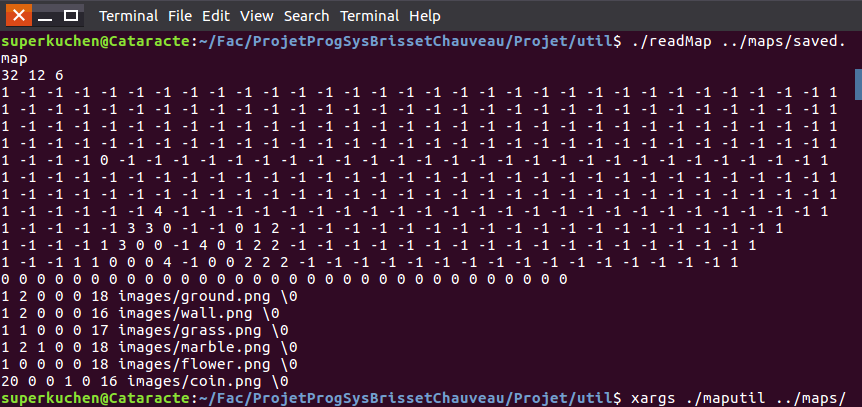
\includegraphics[scale=0.5]{readMap.png} 

Afin de manipuler plus facilement des objets, nous avons défini la structure suivante:
\begin{lstlisting}[language=c]
  typedef struct Object{
    unsigned frames;
    int solid;
    int destructible;
    int collectible;
    int generator;
    int sizeName;
    char* name;
  }Object;
\end{lstlisting}

Pour gérer les nombreuses options disponibles, nous avons utiliser la fonction \textbf{getopt\_long}
\begin{lstlisting}[language=c]
  static struct option long_options[] = {      
    {"getwidth", no_argument, 0,'w'},
    {"getheight", no_argument, 0, 'h'},
    {"getobjects", no_argument, 0, 'o'},
    {"getinfo", no_argument, 0, 'a'},
    {"setwidth",required_argument,0,'W'},
    {"setheight", required_argument, 0,'H'},
    {"setobjects", required_argument, 0, 'O'},
    {"pruneobjects", no_argument, 0, 'p'}
  };
\end{lstlisting}

\subsection{Une erreur surprenante}
L'utilisation de xargs pour l'option \textbf{$-$$-$setobjects} nous a posé dans un premier temps beaucoup de soucis. En effet, pour une raison qui nous est toujours inconnue, l'ordre des premier arguments change lors de l'utilisation de xargs. C'est grâce à l'utilisation de notre fonction de test \textbf{void print\_args( int argc, char** argv);} que nous avons pu observer le phénomène.



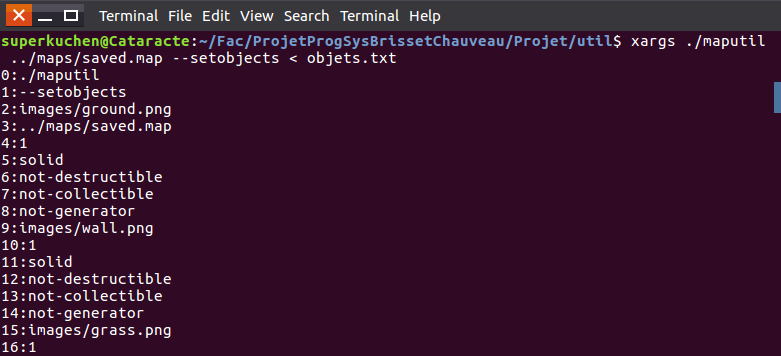
\includegraphics[scale=0.5]{erreurArgs.png}
\\
L'ordre normal des arguments devrait être \textbf{./maputil ../maps/saved.map $-$$-$setobjects images/ground.png ... }

Pour \og résoudre \fg le problème nous avons décidé de régler ce comportement directement en dur dans le code :

\begin{lstlisting}[language=c]
  void args_to_objects(Object** Objets, int argc, char** argv){
    unsigned tmpFra;
    int tmpSol;
    int tmpDestruct;
    int tmpCol;
    int tmpGen;
    int tmpSize;
    char* tmpName;
    for(int i = 3, j = 0; i < argc-1; i += 6, j++){
      if (i != 3){
        tmpName = argv[i];
      }
      else tmpName = argv[2];       //Methode manuelle
      tmpSize = strlen(tmpName)+1;    
      tmpFra = atoi(argv[i+1]);
      if (strcmp("destructible", argv[i+3]) == 0){
        tmpDestruct = 1;
      }
\end{lstlisting}

Conséquences: la fonction marche parfaitement seulement si on utilise xargs pour fournir la liste des objets à passer en paramètre.

\section{Conclusion}
Toutes les options de \textbf{./maputil} ont été correctement implémentées et sont fonctionnelles. En revanche, notre code gagnerait à être un peu plus factorisé. 

\part{Gestion des temporisateurs}

\section{Choix d'implémentation}
Pour la temporisation, nous utilisons l'appel systéme \textbf{setitimer()} qui envoie un signal sigalrm pour un temps donné à la fonction par la structure itimer.
\newline La récuperation des signaux se fait via un thread ``démon'' qui, lorsqu'il recoit un signal sigalrm, appelle la fonction \textbf{sdl\_push\_event()} et ensuite émet un signal sigusr1.
\newline La gestion de plusieurs temporisateurs se fait grâce à l'implémentation d'une \textbf{file de priorité} qui nous permet de toujours avoir en tête de file la liste d'évenements qui se termine en premier. Cette liste contient un ou plusieurs événements qui se terminent en même temps ou dans un intervalle de temps proche du premier élément de cette liste .
\newline La fonction \textbf{defiler} est exécutée lors de la réception du signal sigusr1, et permet de supprimer la première liste de la file. Dans le cas où il y a au moins deux éléments dans cette liste la fonction libère le premier évenement et émet un signal sigalrm pour que le démon puisse gérer cette événement . 

\section{Des difficultés}
La première difficulté était de trouver un moyen pour que le thread principal ne recupère pas le sigalrm, mais le thread démon. Cela à vite été résolu grâce à la fonction \textbf{pthread\_sigmask()} qui permet de bloquer différents signaux pour un thread.
\\
\begin{figure}[!h]
  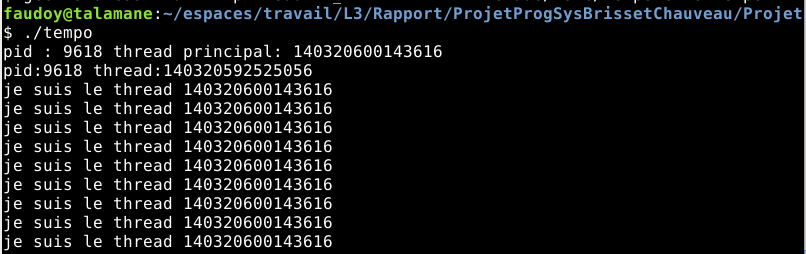
\includegraphics[scale=0.5]{probleme_thread.png}
  \caption{Sans pthread\_sigmask(), le thread princicpal récupére les signaux}  
\end{figure}

Ensuite, une autre difficulté était de bien faire la file de priorité. Ce probléme s'est résolu petit à petit en voyant les erreurs au fûr et à mesure que nous avancions .

Le plus gros probléme a été la succession des temporisations, car nous n'arrivions pas à enchainer les temporisateurs avec la bonne valeur. Nous avons trouvé la solution grâce à l'aide d'un camarade qui nous a aidé à mieux comprendre la succession des temporisateurs, nous n'avions pas bien converti le temps de fin du temporisateur, que nous avions calculé.
\newline
\begin{figure}[!h]
  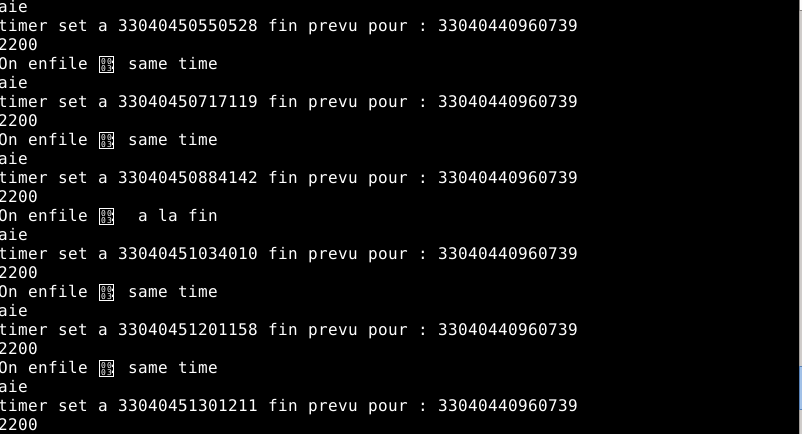
\includegraphics[scale=0.5]{probleme_timer.png}
  \caption{Le timer s'arme à chaque fois qu'on pose une bombe ou une mine}
\end{figure}

\end{document}
